\chapter{Results}

\section{Benchmarks}
\newpage
\subsection{Map tasks}
\begin{figure}[H]
  \centering
  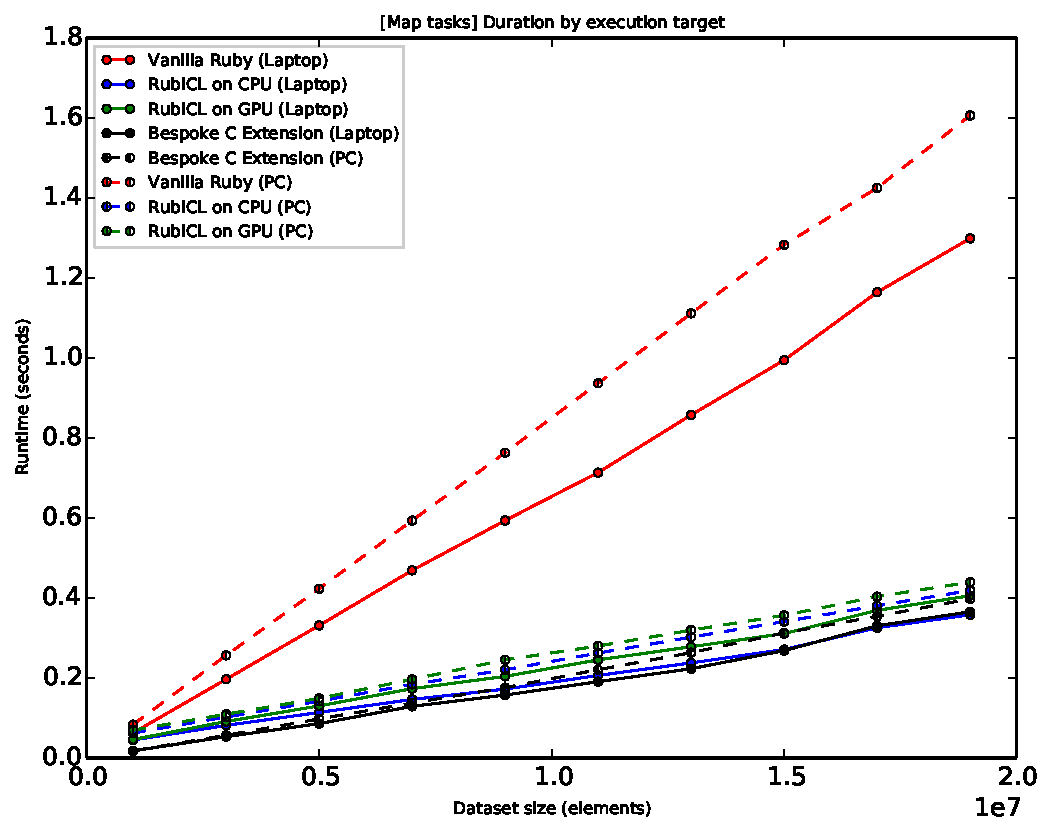
\includegraphics[width=\textwidth]{./graphing/just_map/runtimes.pdf}
  \caption{Task duration by execution target for \emph{Map}.}
  \label{fig:map_task_runtime_g}

  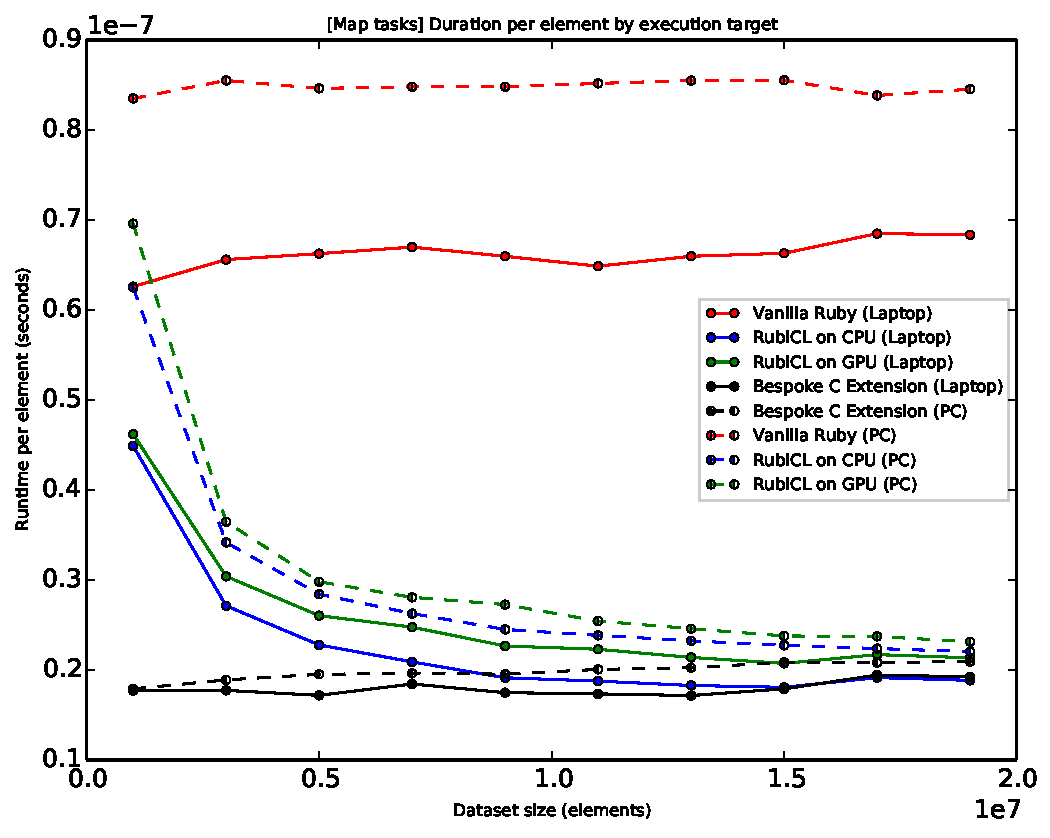
\includegraphics[width=\textwidth]{./graphing/just_map/per_element.pdf}
  \caption{Task duration per processed element for \emph{Map}.}
  \label{fig:map_task_per_el_g}

\end{figure}
\begin{figure}[H]
  \centering
  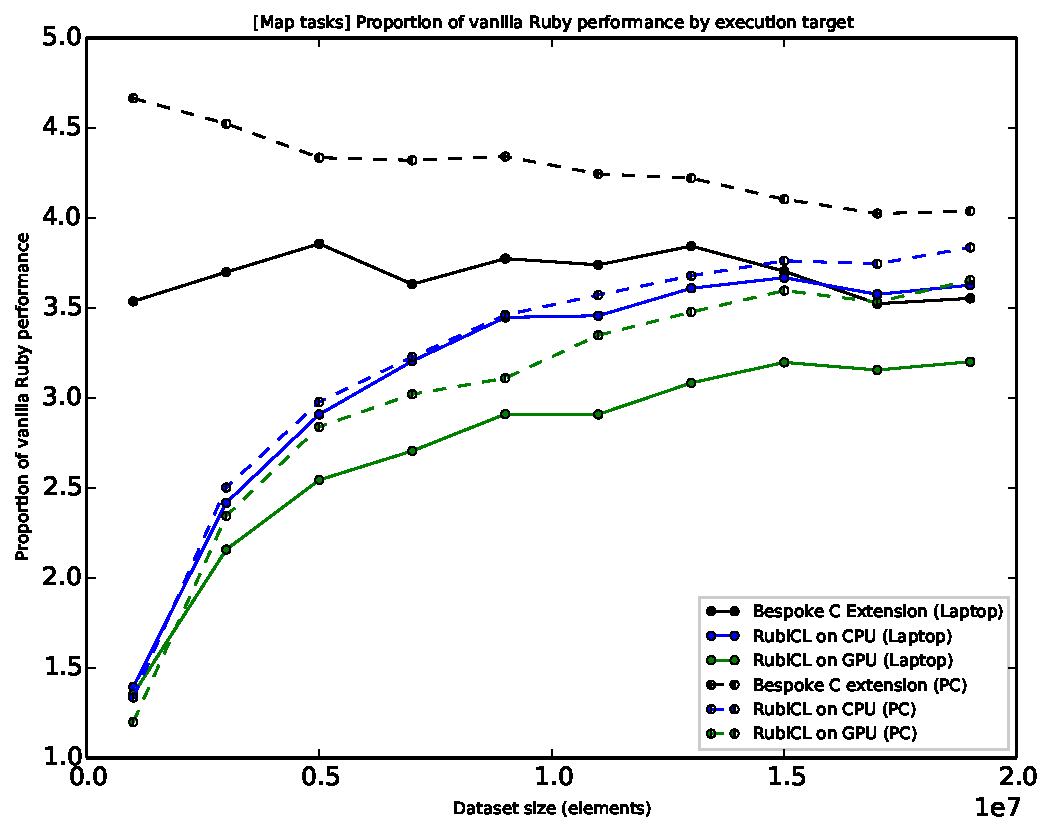
\includegraphics[width=\textwidth]{./graphing/just_map/prop_van.pdf}
  \caption{Proportion of vanilla Ruby performance achieved for \emph{Map}.}
  \label{fig:map_task_vperf_g}

  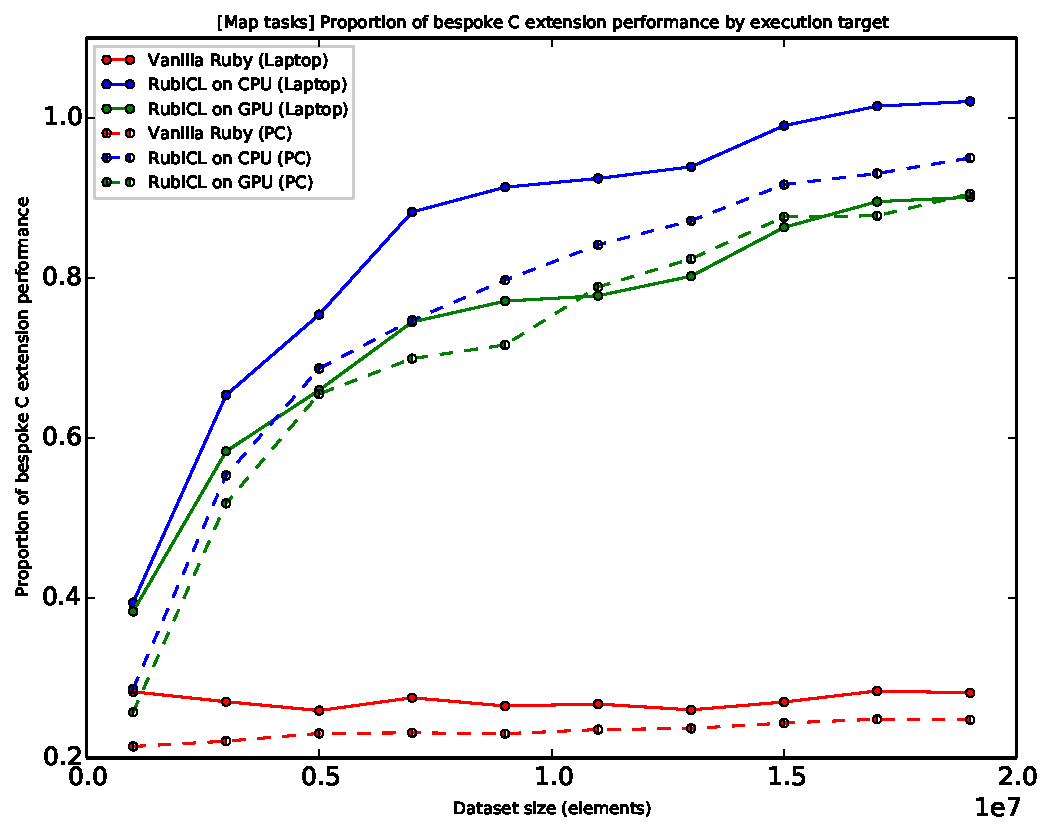
\includegraphics[width=\textwidth]{./graphing/just_map/prop_bes.pdf}
  \caption{Proportion of bespoke C extension performance achieved for \emph{Map}.}
  \label{fig:map_task_bperf_g}
\end{figure}
\subsubsection{Recap of operation performed}
The dense \emph{Map} task performed was the equivalent of \verb!#map { |x| x + 1 }!. This has the effect of incrementing every member of the input dataset.
Performing little work in the supplied function body produces a worst-case evaluation of library performance. This is because performing more work will allow increased throughput to mask any increased latency that the system has. Many tasks will be more involved than incrementation, and very few less so. A result showing that the library is beneficial here should apply even more to all tasks that are of greater intensity.

\subsubsection{Observations and analysis}
Figure~\ref{fig:map_task_runtime_g} shows that all trialled alternatives exhibit similar performance when executing \emph{Map} tasks.
This is likely due to the computational simplicity of the task. The probable cause for the bottleneck is the need to move data in and out of the RubyVM's internal array structures.
Although the gap is slight, the \ac{CPU} compute-devices installed in both machines outperform the \acp{GPGPU} over the range of tested datasets. This is easiest to observe in Figure~\ref{fig:map_task_per_el_g}.

When parallelising purely-map tasks, the project library performs favourably compared to the standard \verb|Enumerable#map| implementation of Ruby $2.2$. Figure~\ref{fig:map_task_vperf_g} demonstrates that, at best, a factor $3.5$\textendash$4$ speed-up over typical execution can be achieved on both systems.
The figure also shows that for all tested datasets, the smallest of which contained $1$ million elements, outsourcing computation to the library was beneficial.

In Figure~\ref{fig:map_task_bperf_g}, it can be seen that on both systems RubiCL throughput is not far from bespoke sequential code. On the laptop, the parallel \ac{CPU} implementation exceeds the non-parallel native extension. It achieves $1.02$ times the rate of processing on $19$ million elements.
However, while the laptop \ac{CPU} presents $4$ hardware threads to \ac{OpenCL}, the native extension utilises only a single thread of execution. As both implementations are performing roughly the same number of operations, it appears that here \ac{OpenCL}'s raw throughput increase is insignificant after processing-model overhead is accounted for.

It is clear that the throughput with which Ruby is capable of performing \emph{Map} tasks has been significantly increased.
On the other hand, the project's parallel library does not significantly outperform a custom, tailored, sequential solution.
Yet, for all systems choosing the optimal device, no less than $80\%$ of the best-presented throughput is achieved at $10$ million elements, improving to no less than $95\%$ at $19$ million.
With the library providing automatic translation of all functions stated into parallel execution patterns, this deficit is insignificant. Much more significant is the mitigation of the need to write and compile native extensions for every required calculation.

\todo{Smaller scale results for all primitives}

\subsection{Dense Filter tasks}
\begin{figure}[H]
  \centering
  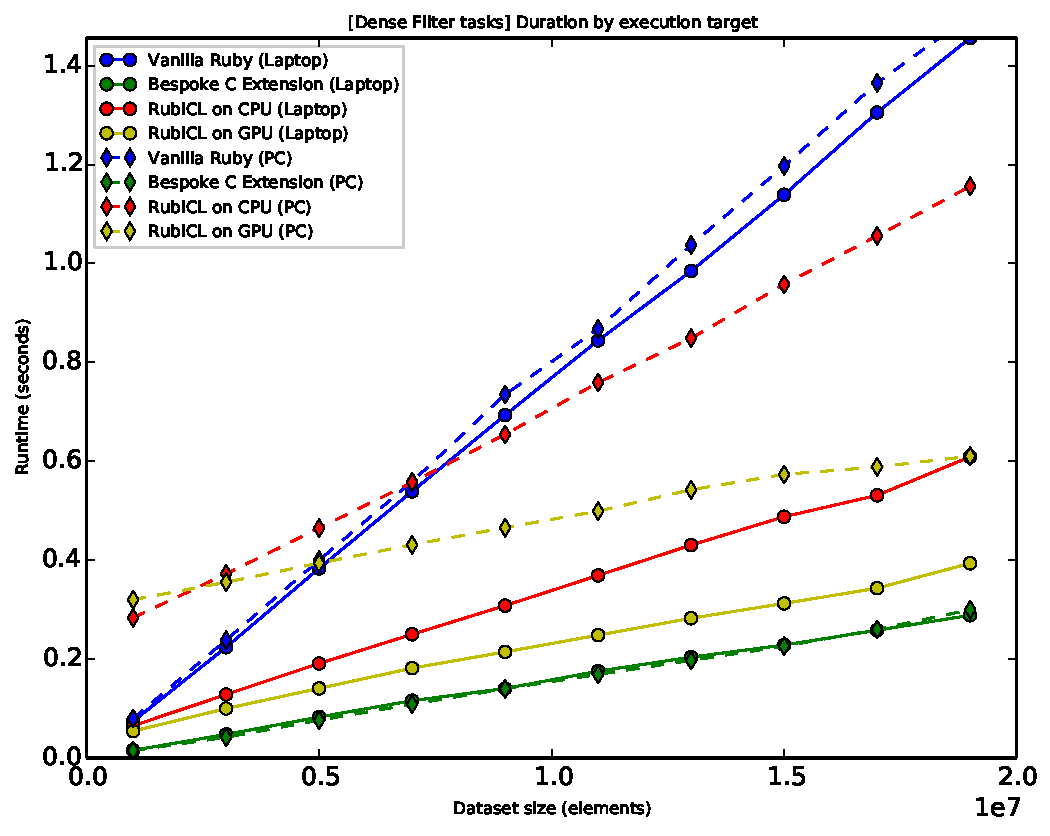
\includegraphics[width=\textwidth]{./graphing/dense_filter/runtimes.pdf}
  \caption{Task duration by execution target for dense \emph{Filter}.}
  \label{fig:dfilter_task_runtime_g}

  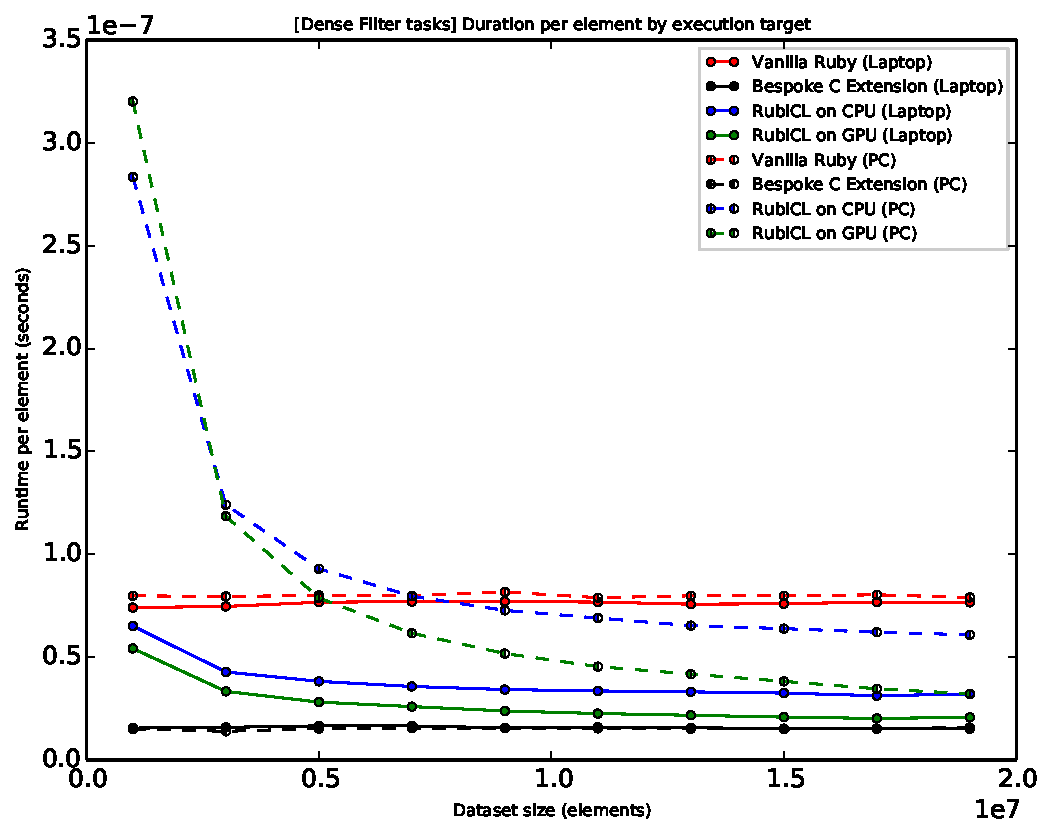
\includegraphics[width=\textwidth]{./graphing/dense_filter/per_element.pdf}
  \caption{Task duration per processed element for dense \emph{Filter}.}
  \label{fig:dfilter_task_per_el_g}

\end{figure}

\begin{figure}[H]
  \centering
  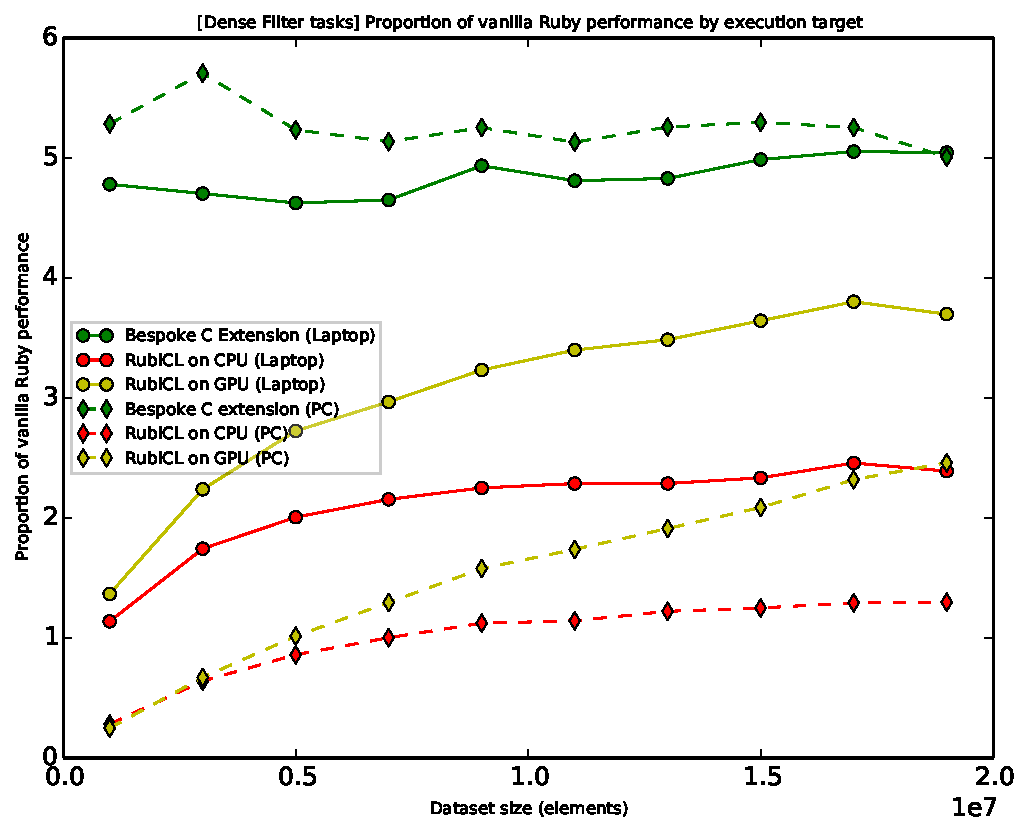
\includegraphics[width=\textwidth]{./graphing/dense_filter/prop_van.pdf}
  \caption{Proportion of vanilla Ruby performance achieved for dense \emph{Filter}.}
  \label{fig:dfilter_task_vperf_g}

  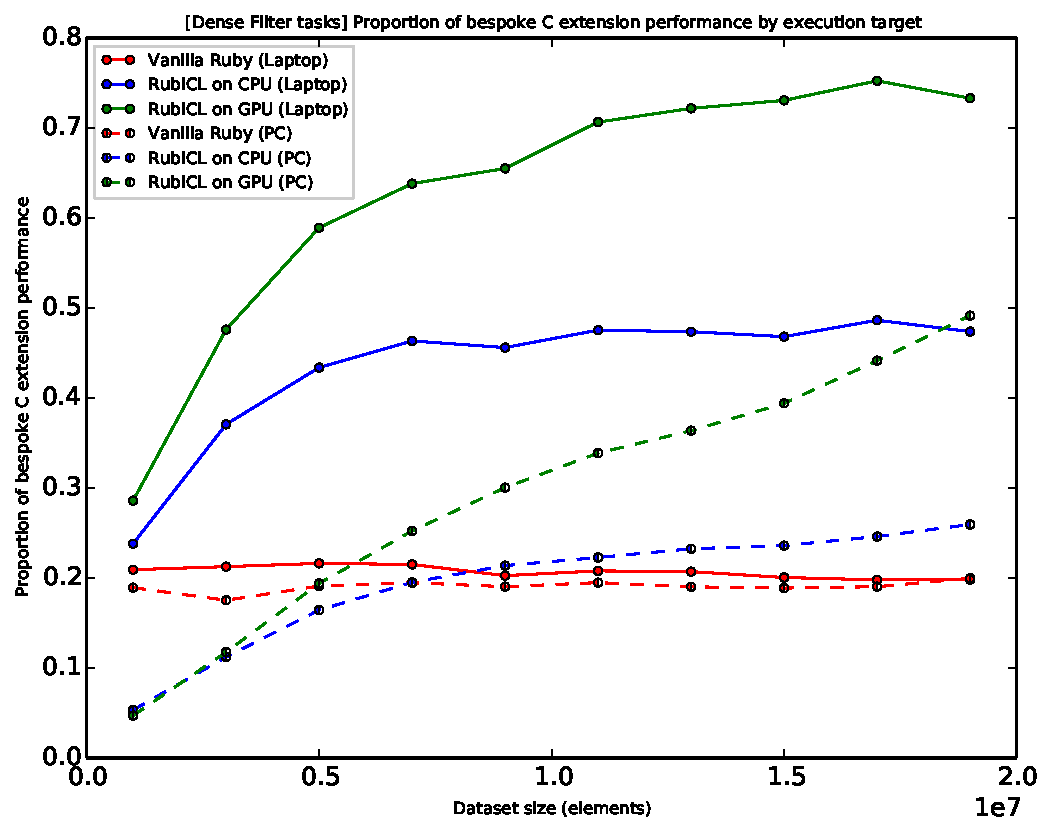
\includegraphics[width=\textwidth]{./graphing/dense_filter/prop_bes.pdf}
  \caption{Proportion of bespoke C extension performance achieved for dense \emph{Filter}.}
  \label{fig:dfilter_task_bperf_g}
\end{figure}
\subsubsection{Recap of operation performed}
The dense \emph{Filter} task performed was the equivalent of \verb!#select { |x| x.even? }!. With the ascending range of data supplied, this will return a subset of the input dataset with half the number of elements.

\subsubsection{Observations and analysis}
Figure~\ref{fig:dfilter_task_runtime_g} is less cluttered than the corresponding graph for \emph{Map} tasks, as there is more variation between the performance of dense \emph{Filter} implementations.
The figure suggests that \emph{Filter} tasks scheduled on the desktop system suffer from a higher latency than their counterparts on the laptop. This is signified by the comparatively elevated runtime for smaller datasets.

Further unlike \emph{Map} tasks, on both systems the \ac{GPGPU} compute-device outperforms the \ac{CPU} when filtering large datasets. For the laptop system, the domination is present on every tested dataset size. On the contrary, the desktop \ac{CPU} is initially a shade faster but is quickly dwarfed by the significantly higher throughput of the \ac{GPGPU} device.

On the laptop system, Figure~\ref{fig:dfilter_task_vperf_g} demonstrates that the library is beneficial when processing all datasets within the tested range. The desktop is not quite as successful at performing dense purely-\emph{Filter} tasks, hampered when producing subsets of smaller datasets by its increased latency. At least $5$ million elements are required before it is worthwhile to offload computation onto the \ac{GPGPU} via RubiCL. The \ac{CPU} trails not long after, at $8$ million elements, but never achieves more than $25\%$ speedup over the standard Ruby implementation.

On both test systems, when using the \ac{GPGPU}, noticeable speedup of \emph{Filter} operations can be achieved. With a $2.5$ times speedup on the desktop and over $3.5$ times on the laptop, large filtering operations are significantly accelerated by the RubiCL library.

Figure~\ref{fig:dfilter_task_bperf_g} shows that the laptop \ac{GPGPU} achieves a high proportion, peaking at $75\%$, of bespoke sequential code performance. The desktop system boasts a lesser proportion, at $50\%$, but the lack of plateau in the figure suggests that this gap would close further as datasets increase in size.

The lacklustre performance for \ac{CPU} devices can be partly explained by the fact that the parallel implementation of filtering, although asymptotically identical in cost, requires much more work than a sequential filter. In this case, the hidden constants involved for distributing computation have a large effect on the task duration, larger than that of parallelising the predicate scan along the data.

This reasoning can also explain why the \ac{GPGPU} devices fail to outperform the custom extension over the given range of datasets.
Nonetheless, the need to write and compile native extensions for each distinct query performed is again removed when using the RubiCL library. A system-dependent performance hit of between $25\%$ and $50\%$ behind a handwritten extension is far more justifiable when it facilitates rapid-prototyping, especially when compared to the $80\%$ penalty that Figure~\ref{fig:dfilter_task_bperf_g} highlights for unoptimised Ruby $2.2$.

\subsection{Sparse Filter tasks}
\begin{figure}[H]
  \centering
  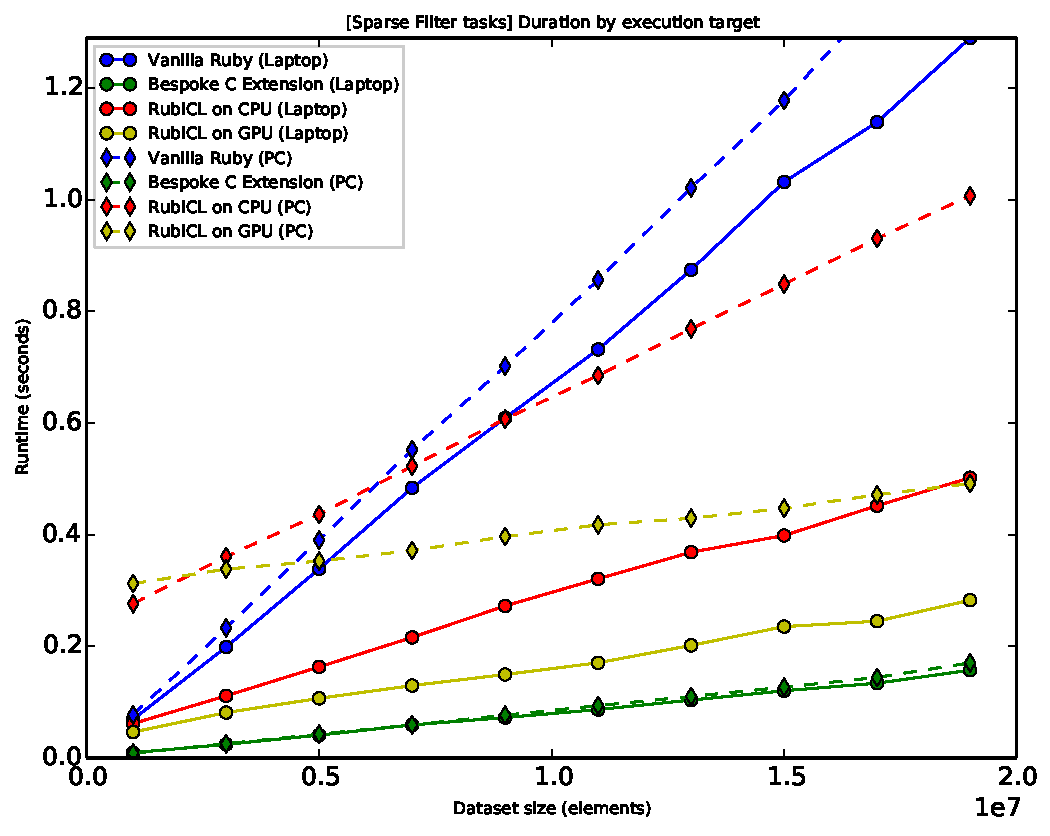
\includegraphics[width=\textwidth]{./graphing/sparse_filter/runtimes.pdf}
  \caption{Task duration by execution target for sparse \emph{Filter}.}
  \label{fig:sfilter_task_runtime_g}

  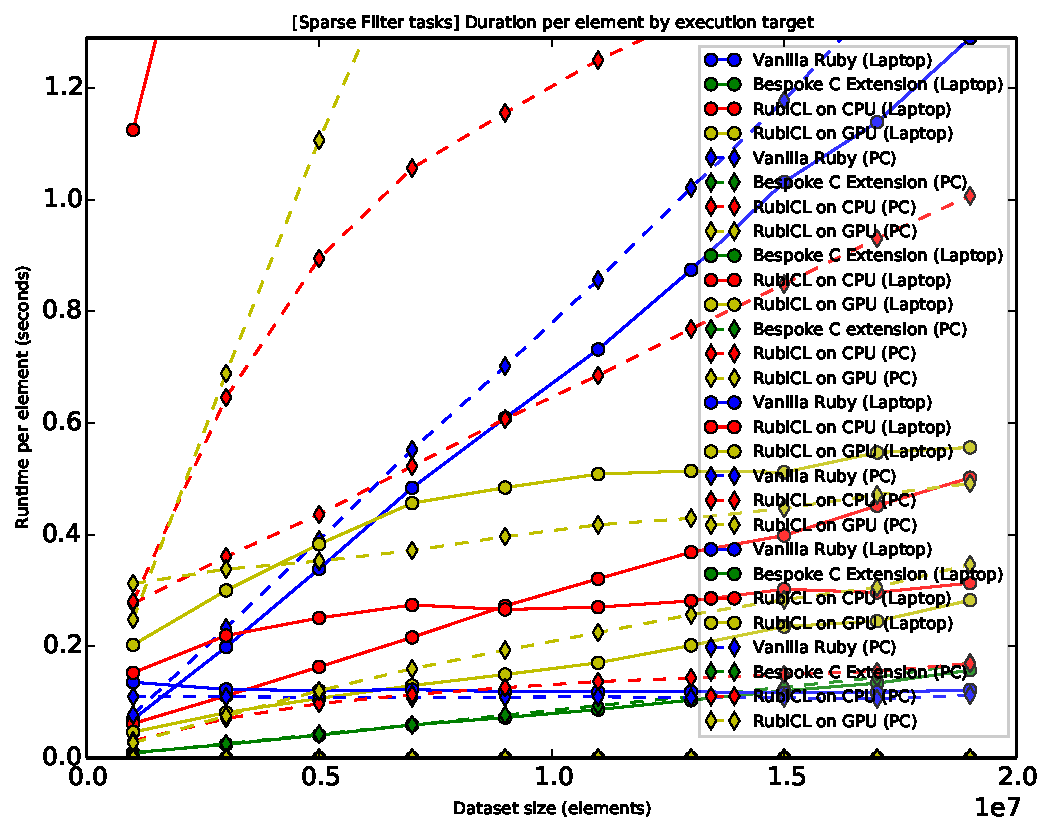
\includegraphics[width=\textwidth]{./graphing/sparse_filter/per_element.pdf}
  \caption{Task duration per processed element for sparse \emph{Filter}.}
  \label{fig:sfilter_task_per_el_g}

\end{figure}

\begin{figure}[H]
  \centering
  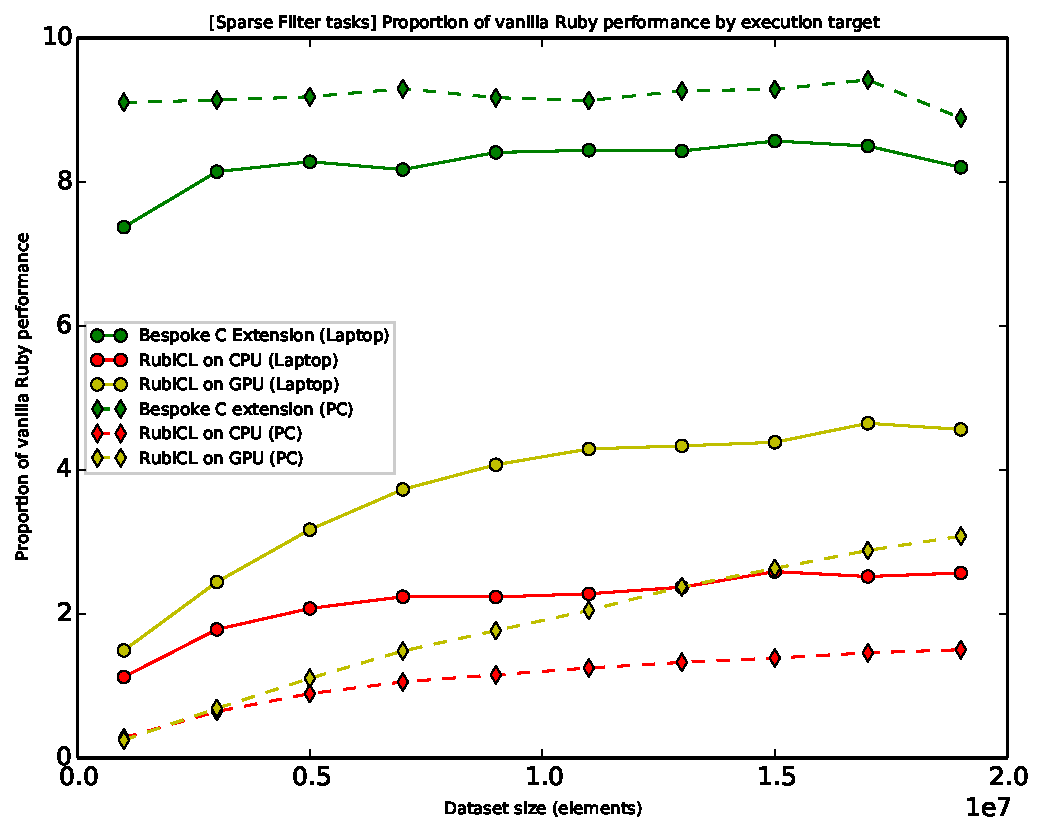
\includegraphics[width=\textwidth]{./graphing/sparse_filter/prop_van.pdf}
  \caption{Proportion of vanilla Ruby performance achieved for sparse \emph{Filter}.}
  \label{fig:sfilter_task_vperf_g}

  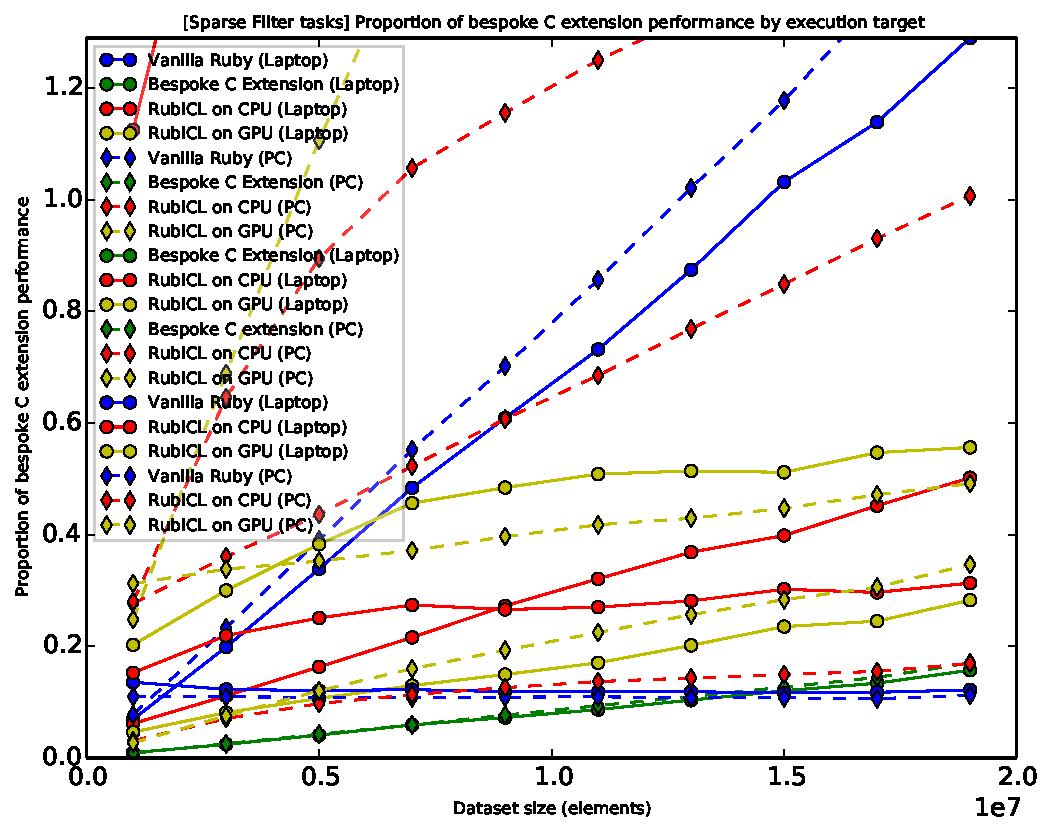
\includegraphics[width=\textwidth]{./graphing/sparse_filter/prop_bes.pdf}
  \caption{Proportion of bespoke C extension performance achieved for sparse \emph{Filter}.}
  \label{fig:sfilter_task_bperf_g}
\end{figure}
\subsubsection{Recap of operation performed}
The sparse \emph{Filter} task, returning fewer elements than the dense task, performed was the equivalent of \verb!#select { |x| x % 20 == 0 }!. This selects all elements that are evenly divisible by 20. With the ascending range of data supplied, this will return a subset of the input dataset with $5\%$ of its elements remaining.

\subsubsection{Observations and analysis}
Figure~\ref{fig:sfilter_task_runtime_g} looks very similar to that of dense filtering. Indeed, many of the observations are the same.
One reason for this is that none of the code benchmarked, including \verb|Enumerable#select|, changes behaviour when datasets are sparse.
Instead, the slight change in performance can be explained by differing proportions of time spent inserting elements or transferring device datasets when the set of returned results is smaller in size.

As before, the difference in latency between the laptop and desktop systems causes a significant proportional gap for smaller datasets.
It leaves sparse \emph{Filter} needing the same minimum dataset sizes for beneficial inclusion as dense \emph{Filter}.
This identical result is useful as it suggests that the threshold for parallelisation can be estimated without prior knowledge of the proportion of data retained.

Yet again, \ac{GPGPU} devices are dominant among the \ac{OpenCL} filtering implementations, for all but the smallest dataset on the desktop.
Much like the previous graph for filtering, the desktop \ac{GPGPU} does not appear to have plateaued in time-per-element. Therefore, further study should be performed to see at what size dataset this occurs.

The bespoke extension performs much better comparatively at sparse filtering than dense filtering. Figure~\ref{fig:sfilter_task_vperf_g} shows a $9$ times performance speedup over unoptimised code, nearly twice the speedup of dense filtering.
With this in mind, Figure~\ref{fig:sfilter_task_bperf_g} shows a decrease in performance of RubiCL relative to bespoke filtering, compared to the denser predicate examined earlier.

The inverse is true in Figure~\ref{fig:sfilter_task_vperf_g}, with RubiCL demonstrating an improved $3$\textendash$5$ times speedup when executing on \ac{GPGPU} devices over Ruby $2.2$ for dense filtering.
The differences in relative performance between dense and sparse \emph{Filter} task implementations suggest that the cause for diverging ratios may result from there being fewer conditional insertions to the result vector. Alternatively, when less data is returned from a compute-device, the one-off latency penalty is more significant and may offset the benefits of relatively-high transfer bandwidth.

\subsection{MapFilter tasks}
\begin{figure}[H]
  \centering
  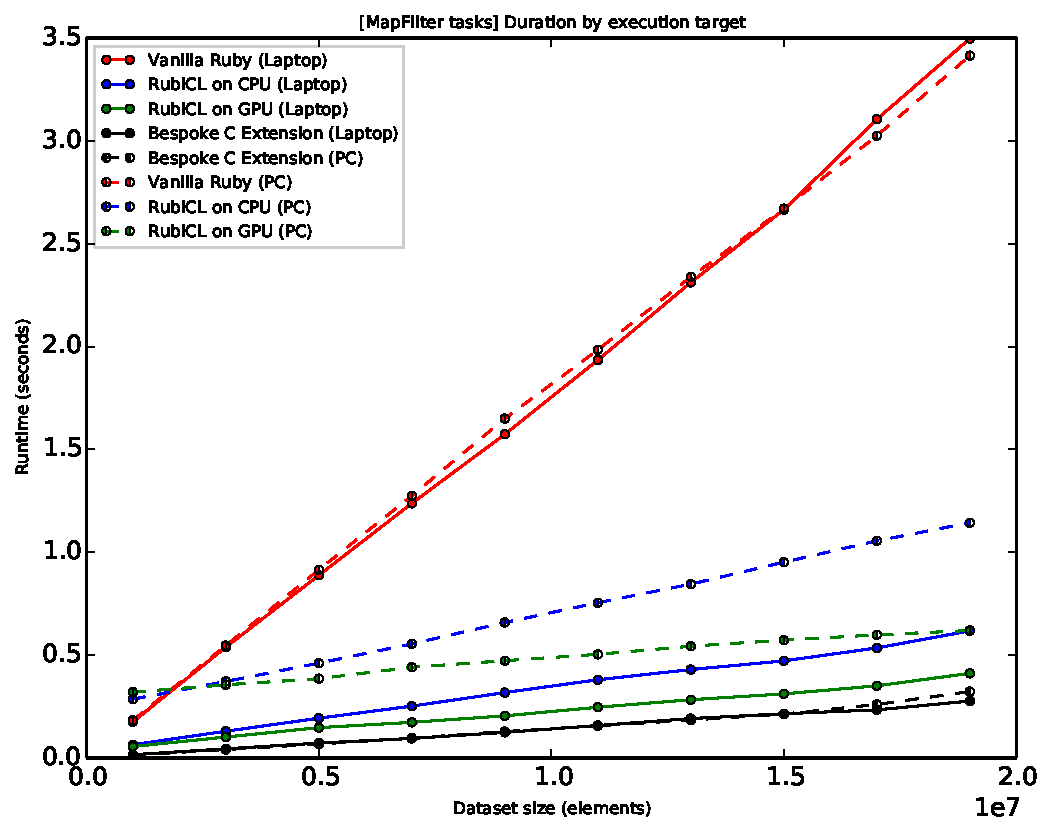
\includegraphics[width=\textwidth]{./graphing/mapfilter/runtimes.pdf}
  \caption{Task duration by execution target for \emph{MapFilter}.}
  \label{fig:mfilter_task_runtime_g}

  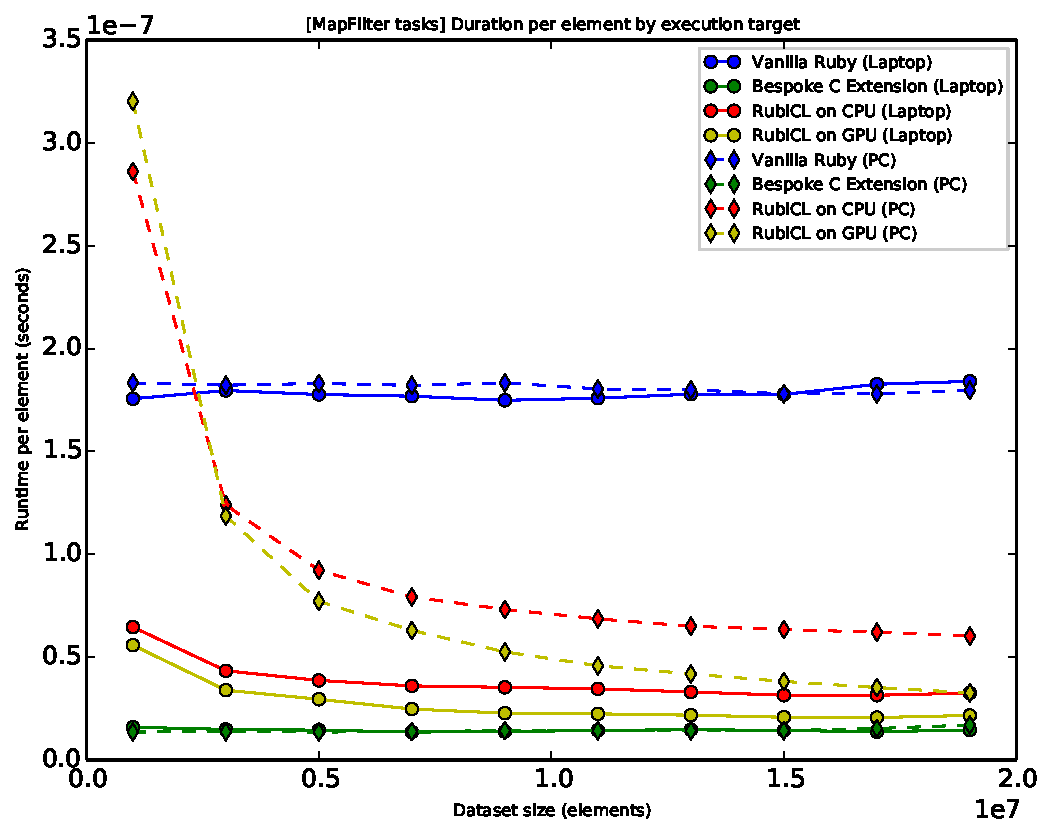
\includegraphics[width=\textwidth]{./graphing/mapfilter/per_element.pdf}
  \caption{Task duration per processed element for \emph{MapFilter}.}
  \label{fig:mfilter_task_per_el_g}

\end{figure}

\begin{figure}[H]
  \centering
  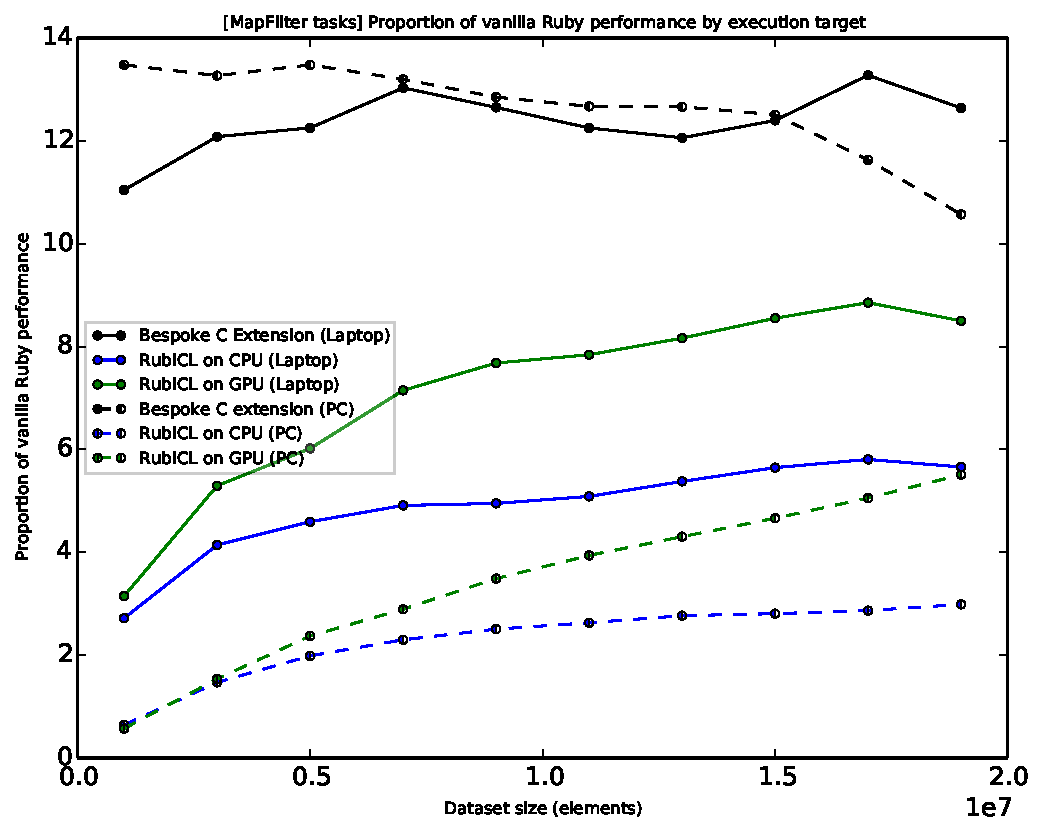
\includegraphics[width=\textwidth]{./graphing/mapfilter/prop_van.pdf}
  \caption{Proportion of vanilla Ruby performance achieved for \emph{MapFilter}.}
  \label{fig:mfilter_task_vperf_g}

  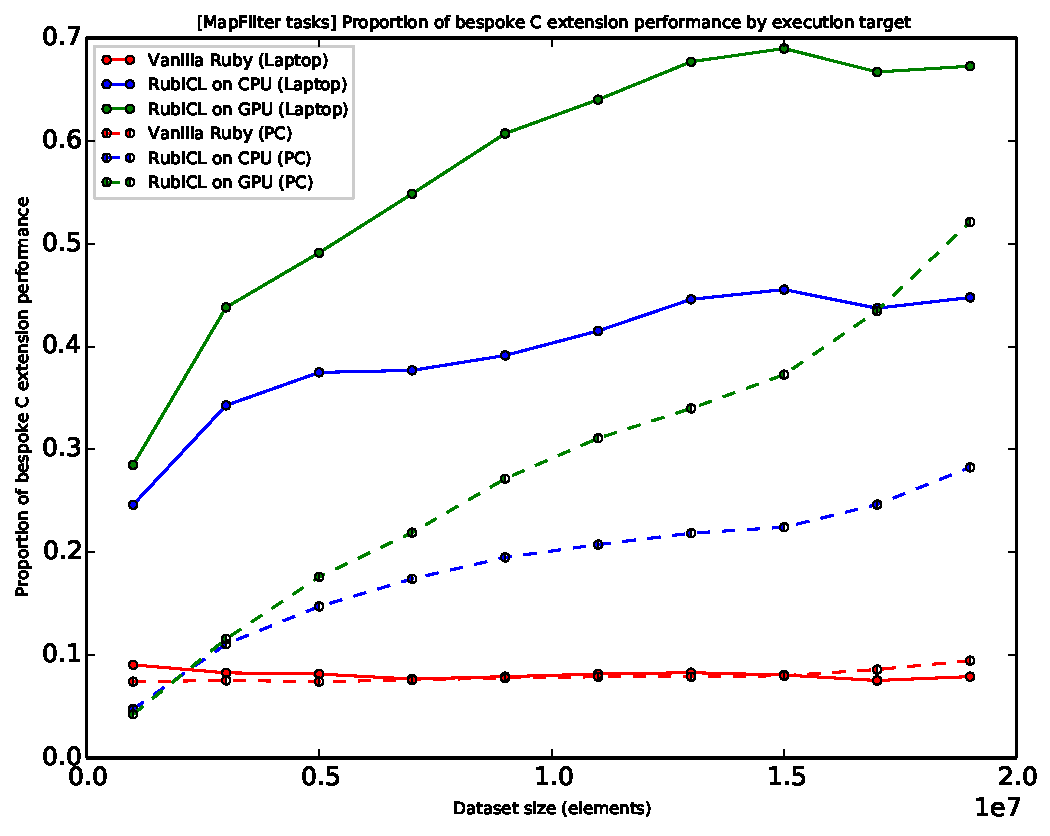
\includegraphics[width=\textwidth]{./graphing/mapfilter/prop_bes.pdf}
  \caption{Proportion of bespoke C extension performance achieved for \emph{MapFilter}.}
  \label{fig:mfilter_task_bperf_g}
\end{figure}
\subsubsection{Recap of operation performed}
The computation pipeline for this benchmark consisted of the earlier \emph{Map} task, immediately followed by the dense \emph{Filter} task.
This has the combined effect of incrementing all elements and then returning the subset of mutated elements that are even.
Again this returns a dataset that is half of the original size. Furthermore, the tasks can undergo \emph{fusion} in order to reduce the number of kernels scheduled and required passes over the data.


\subsubsection{Observations and analysis}
When a \emph{Map} task is followed by a \emph{Filter} task, the project's task fusion optimisation drastically improves performance.
Figure~\ref{fig:mfilter_task_runtime_g} demonstrates how significantly runtime diverges, with the gap between Ruby $2.2$ and competing implementations expanding greatly as larger datasets are introduced.
The need for multiple passes over the data greatly delays the unoptimised code, as intermediate yet discarded results for the method pipeline are computed.
The optimisation can be seen to reduce the minimum dataset length required for RubiCL's desktop parallelism to provide performance gains over the standard implementation, shown in Figure~\ref{fig:mfilter_task_vperf_g}. At just $2$ million elements, it is less than half of that required when filtering alone.

Figure~\ref{fig:mfilter_task_vperf_g} also demonstrates the significant throughput increases provided by RubiCL, compared to the standard library. At over $8$ times speedup, combining subsequent \emph{Map} and \emph{Filter} tasks then dispatching the computation to the \ac{GPGPU} can speed up laptop computation greatly. At nearly $5$ times speedup, and the proportional graph again showing no sign of plateau, the same tactic is also highly beneficial on the desktop system used for testing.

\ac{GPGPU} devices continue to dominate \ac{CPU} devices, as with other \emph{Filter} tasks. This occurs even though a \emph{Map} task, something that \ac{CPU} architecture excelled at earlier, has been prepended. It is possible that the simpler task performed earlier did not benefit from the improved device throughput, once the latency cost of context-switching computation was introduced.

Comparison with a bespoke sequential solution in Figure~\ref{fig:mfilter_task_bperf_g} shows that a large proportion of tailored solution performance is obtained on both systems.
The laptop system obtains, at best, $70\%$ performance and the desktop system obtains $50\%$ with further indications of increasing proportion on larger datasets.
This is even more significant as the manual fusion process of custom extension development is conceptually more involved than distinct tasks.
As more mutation and filtering conditionals are brought into the loop body, the compiler is able to eradicate more redundant computation but the source code becomes harder to interpret correctly. With RubiCL's task fusion, separately stated pipeline stages are less concept-dense and therefore easier to understand.

\todo{Scan task results and flop}

\section{User evaluation}
